%!Mode:: "TeX:UTF-8"
\documentclass[a4paper,11pt,UTF8]{ctexart}
\usepackage{indentfirst} %缩进
\usepackage{xeCJK}    %使用系统字体
\usepackage{fancyhdr} %自定义页眉页脚
\pagestyle{empty}                   %不设置页眉页脚
\usepackage{amsmath, amsthm, amssymb, amsfonts} %数学公式
\usepackage[a4paper,left=3cm,right=3cm,top=3cm,bottom=3cm]{geometry}
%\usepackage[tmargin=1in,bmargin=1in,lmargin=1.25in,rmargin=1.25in]{geometry}.
\usepackage{booktabs} %插入表格
\usepackage[section]{placeins} %避免浮动
\usepackage{listings} %插入代码
\usepackage{ctex}     %中文宏包
\usepackage[svgnames, table]{xcolor} %彩色表格
\usepackage{algorithm}          %伪代码
\usepackage{algorithmicx}
\usepackage{algpseudocode}
\usepackage{algorithm,algpseudocode,float}
\usepackage{lipsum}
\usepackage{enumitem}           %调整列举环境
\usepackage{url}
\usepackage{fontspec,xunicode}
\usepackage{cite}
\defaultfontfeatures{Mapping=tex-text} %如果没有它,会有一些 tex 特殊字符无法正常使用,比如连字符。

\usepackage{graphicx}
\usepackage{subfigure}
\graphicspath{{imgs/}}

%%%%%%%%%%%%%%%%%%%%%%%%%%%%%%%%%%%%%%%%%%%%%%%%%%%%%%%%%%%%%%%%
% 缩进及行间距
%%%%%%%%%%%%%%%%%%%%%%%%%%%%%%%%%%%%%%%%%%%%%%%%%%%%%%%%%%%%%%%%
\setlength{\parindent}{22pt} %重新定义缩进长度
\setlength{\baselineskip}{20pt}  %定义行间距
%\renewcommand{\baselinestretch}{1.1} %定义行间距

%%%%%%%%%%%%%%%%%%%%%%%%%%%%%%%%%%%%%%%%%%%%%%%%%%%%%%%%%%%%%%%%
% 列表设置
%%%%%%%%%%%%%%%%%%%%%%%%%%%%%%%%%%%%%%%%%%%%%%%%%%%%%%%%%%%%%%%%
\setenumerate{fullwidth,itemindent=\parindent,listparindent=\parindent,itemsep=0ex,partopsep=0pt,parsep=0ex}
\setenumerate[2]{label=\alph*),leftmargin=1.5em}  %二级item设置
\setitemize{itemindent=38pt,leftmargin=0pt,itemsep=-0.4ex,listparindent=26pt,partopsep=0pt,parsep=0.5ex,topsep=-0.25ex}
\setdescription{itemindent=38pt,leftmargin=0pt,itemsep=-0.4ex,listparindent=26pt,partopsep=0pt,parsep=0.5ex,topsep=-0.25ex}

%%%%%%%%%%%%%%%%%%%%%%%%%%%%%%%%%%%%%%%%%%%%%%%%%%%%%%%%%%%%%%%%
% 图的标题行间距设置
%%%%%%%%%%%%%%%%%%%%%%%%%%%%%%%%%%%%%%%%%%%%%%%%%%%%%%%%%%%%%%%%
\newcommand{\bottomcaption}{%
\setlength{\abovecaptionskip}{6pt}%
\setlength{\belowcaptionskip}{6pt}%
\caption}


%%%%%%%%%%%%%%%%%%%%%%%%%%%%%%%%%%%%%%%%%%%%%%%%%%%%%%%%%%%%%%%%
% 字体定义
%%%%%%%%%%%%%%%%%%%%%%%%%%%%%%%%%%%%%%%%%%%%%%%%%%%%%%%%%%%%%%%%
\setmainfont{Times New Roman}  %默认英文字体.serif是有衬线字体sans serif无衬线字体
\setmonofont{Consolas}
\setCJKmainfont[ItalicFont={楷体}, BoldFont={黑体}]{宋体}%衬线字体 缺省中文字体为
\setCJKsansfont{黑体}
\punctstyle{hangmobanjiao}
%-----------------------xeCJK下设置中文字体------------------------------%
\setCJKfamilyfont{song}{SimSun}                             %宋体 song
\newcommand{\song}{\CJKfamily{song}}
\setCJKfamilyfont{fs}{FangSong}                      %仿宋  fs
\newcommand{\fs}{\CJKfamily{fs}}
\setCJKfamilyfont{ktgb}{KaiTi}                      %楷体2312 ktgb
\newcommand{\ktgb}{\CJKfamily{ktgb}}
\setCJKfamilyfont{yh}{Microsoft YaHei}                    %微软雅黑 yh
\newcommand{\yh}{\CJKfamily{yh}}
\setCJKfamilyfont{hei}{SimHei}                              %黑体  hei
\newcommand{\hei}{\CJKfamily{hei}}
\setCJKfamilyfont{hwxk}{STXingkai}                                %华文行楷  hwxk
\newcommand{\hwxk}{\CJKfamily{hwxk}}
%------------------------------设置字体大小------------------------%
\newcommand{\shiyanbaogao}{\fontsize{36pt}{\baselineskip}\selectfont}
\newcommand{\chuhao}{\fontsize{42pt}{\baselineskip}\selectfont}     %初号
\newcommand{\xiaochuhao}{\fontsize{36pt}{\baselineskip}\selectfont} %小初号
\newcommand{\yihao}{\fontsize{28pt}{\baselineskip}\selectfont}      %一号
\newcommand{\erhao}{\fontsize{21pt}{\baselineskip}\selectfont}      %二号
\newcommand{\xiaoerhao}{\fontsize{18pt}{\baselineskip}\selectfont}  %小二号
\newcommand{\sanhao}{\fontsize{15.75pt}{\baselineskip}\selectfont}  %三号
\newcommand{\sihao}{\fontsize{14pt}{\baselineskip}\selectfont}       %四号
\newcommand{\xiaosihao}{\fontsize{12pt}{\baselineskip}\selectfont}  %小四号
\newcommand{\wuhao}{\fontsize{10.5pt}{\baselineskip}\selectfont}    %五号
\newcommand{\xiaowuhao}{\fontsize{9pt}{\baselineskip}\selectfont}   %小五号
\newcommand{\liuhao}{\fontsize{7.875pt}{\baselineskip}\selectfont}  %六号
\newcommand{\qihao}{\fontsize{5.25pt}{\baselineskip}\selectfont}    %七号

%%%%%%%%%%%%%%%%%%%%%%%%%%%%%%%%%%%%%%%%%%%%%%%%%%%%%%%%%%%%%%%%
% 图题字体大小相同
%%%%%%%%%%%%%%%%%%%%%%%%%%%%%%%%%%%%%%%%%%%%%%%%%%%%%%%%%%%%%%%%
\usepackage{caption}
\captionsetup{font={footnotesize}}   % footnotesize = 9pt
\captionsetup[lstlisting]{font={footnotesize}}

%%%%%%%%%%%%%%%%%%%%%%%%%%%%%%%%%%%%%%%%%%%%%%%%%%%%%%%%%%%%%%%%
% 重定义枚举编号为 1),2)...
%%%%%%%%%%%%%%%%%%%%%%%%%%%%%%%%%%%%%%%%%%%%%%%%%%%%%%%%%%%%%%%%
\renewcommand{\labelenumi}{\theenumi)}


%%%%%%%%%%%%%%%%%%%%%%%%%%%%%%%%%%%%%%%%%%%%%%%%%%%%%%%%%%%%%%%%
% 重定义section标题
%%%%%%%%%%%%%%%%%%%%%%%%%%%%%%%%%%%%%%%%%%%%%%%%%%%%%%%%%%%%%%%%
\CTEXsetup[format={\sihao\CJKfamily{zhhei}\zihao{4}},number={\chinese{section}},name={,、~},aftername={},indent={0pt},beforeskip={6pt},afterskip={6pt},format+={\flushleft}]{section}
\CTEXsetup[format={\Large\bfseries\CJKfamily{zhkai}\zihao{5}},name={(,)},number={\chinese{subsection}},aftername={},indent={22pt},beforeskip={14pt},afterskip={2pt}]{subsection}
\CTEXsetup[number={\chinese{section}},name={附录, ~~ }]{appendix}



%%%%%%%%%%%%%%%%%%%%%%%%%%%%%%%%%%%%%%%%%%%%%%%%%%%%%%%%%%%%%%%%
% 标题名称中文化
%%%%%%%%%%%%%%%%%%%%%%%%%%%%%%%%%%%%%%%%%%%%%%%%%%%%%%%%%%%%%%%%
\renewcommand\figurename{\hei 图}
\renewcommand\tablename{\hei 表}
\renewcommand\lstlistingname{\hei 代码}
\renewcommand{\algorithmicrequire}{\textbf{输入:}}
\renewcommand{\algorithmicensure}{\textbf{输出:}}
\newtheorem{define}{定义}

%%%%%%%%%%%%%%%%%%%%%%%%%%%%%%%%%%%%%%%%%%%%%%%%%%%%%%%%%%%%%%%%
% 代码设置
%%%%%%%%%%%%%%%%%%%%%%%%%%%%%%%%%%%%%%%%%%%%%%%%%%%%%%%%%%%%%%%%
\lstset{
 columns=fixed,
 numbers=left,                                        % 在左侧显示行号
 numberstyle=\tiny\color{gray},                       % 设定行号格式
 frame=single,                                        % 单线背景边框
 breaklines=true,                                     % 设定LaTeX对过长的代码行进行自动换行
 keywordstyle=\color[RGB]{40,40,255},                 % 设定关键字颜色
 numberstyle=\footnotesize\color{darkgray},
 commentstyle=\it\color[RGB]{0,96,96},                % 设置代码注释的格式
 stringstyle=\rmfamily\slshape\color[RGB]{128,0,0},   % 设置字符串格式
 showstringspaces=false,                              % 不显示字符串中的空格
 language=java,                                        % 设置语言
 basicstyle=\linespread{1.0}\xiaowuhao\ttfamily,                      % 字体字号
 %lineskip=10pt,
 %baselinestretch=1,
}

%%%%%%%%%%%%%%%%%%%%%%%%%%%%%%%%%%%%%%%%%%%%%%%%%%%%%%%%%%%%%%%%
% 伪代码分页
%%%%%%%%%%%%%%%%%%%%%%%%%%%%%%%%%%%%%%%%%%%%%%%%%%%%%%%%%%%%%%%%
\makeatletter
\renewcommand{\ALG@name}{算法}
\newenvironment{breakablealgorithm}
  {% \begin{breakablealgorithm}
   \begin{center}
     \refstepcounter{algorithm}% New algorithm
     \hrule height.8pt depth0pt \kern2pt% \@fs@pre for \@fs@ruled
     \renewcommand{\caption}[2][\relax]{% Make a new \caption
       {\raggedright\textbf{\ALG@name~\thealgorithm} ##2\par}%
       \ifx\relax##1\relax % #1 is \relax
         \addcontentsline{loa}{algorithm}{\protect\numberline{\thealgorithm}##2}%
       \else % #1 is not \relax
         \addcontentsline{loa}{algorithm}{\protect\numberline{\thealgorithm}##1}%
       \fi
       \kern2pt\hrule\kern2pt
     }
  }{% \end{breakablealgorithm}
     \kern2pt\hrule\relax% \@fs@post for \@fs@ruled
   \end{center}
  }
\makeatother



\begin{document}
\xiaosihao\song

\begin{titlepage}
\center{\yihao{\ktgb{中山大学数据科学与计算机学院\\操作系统实验课程}}}
\vspace{1cm}


\center{\shiyanbaogao{\ktgb{实~验~报~告}}}
\vspace{2cm}

\begin{center}
\begin{large}
\begin{tabular}{rc}
\xiaoerhao{\hei{教\qquad 师}}& \sanhao{\hei{凌应标}}\\
\cline{2-2}\\
\xiaoerhao{\hei{学\qquad 号}}& \hspace{1.7cm}\sanhao{\hei{17341035\hspace{1.7cm}}} \\
\cline{2-2}\\
\xiaoerhao{\hei{姓\qquad 名}}& \sanhao{\hei{傅畅}}\\
\cline{2-2}\\
\xiaoerhao{\hei{实验名称}}& \sanhao{\hei{实验四(异步事件编程)}}\\
\cline{2-2}\\

\end{tabular}
\end{large}
\end{center}
\vfill \hfill
\end{titlepage}
\clearpage

\centerline{\\[10pt]\erhao{\fs{实~验~四}}}
\centerline{\\[10pt]\yihao{\fs{异~步~事~件~编~程}}}

\leftline{\\[8pt]\xiaosihao{\hei{\hspace{1.5em} 姓名:傅畅\hfill 学号:17341038 \hfill  }}}

\leftline{\\[8pt]\xiaosihao{\hei{\hspace{1.5em} 邮箱:fuch8@mail2.sysu.edu.cn \hfill}}}

\leftline{\\[8pt]\xiaosihao{\hei{\hspace{1.5em} 实验时间:周五(3-4节) \hfill }}}


\setcounter{tocdepth}{2}
\setlength{\parskip}{0pt}
\tableofcontents
\clearpage


\section{实验要求}

	\subsection{利用时钟中断,在右下角轮流显示转轮}

	操作系统工作期间,利用时钟中断,在屏幕24行79列位置轮流显示’|’、’/’和'$\backslash$',适当控制显示速度,以方便观察效果。

	\subsection{编写键盘中断响应程序}
	编写键盘中断响应程序,原有的你设计的用户程序运行时,键盘事件会做出有事反应:当键盘有按键时,屏幕适当位置显示”OUCH! OUCH!”。
	\subsection{编写软中断服务程序}
	在内核中,对33号、34号、35号和36号中断编写中断服务程序,分别在屏幕1/4区域内显示一些个性化信息。再编写一个汇编语言的程序,作为用户程序,利用int 33、int 34、int 35和int 36产生中断调用你这4个服务程序。

\section{实验配置}

	\subsection{实验支撑环境}
		\begin{itemize} 
			\item 硬件:个人计算机
			\item 主机操作系统:Linux 4.18.0-16-generic 17-Ubuntu
			\item 虚拟机软件: Bochs 2.6.9
		\end{itemize}
	
	
	 
\section{x86保护模式学习}
	\subsection{使用选择子访存}
	选择子在
	\subsection{分页机制}

	\subsection{中断选择子}

	% \lstset{language=={[x86nasm]Assembler}}
	% \begin{lstlisting}[caption={},tabsize=4,basicstyle=\footnotesize,captionpos=b]
	
	% \end{lstlisting}
	

\section{实验代码设计}
	\subsection{从软盘到使用硬盘启动}
	由于使用空间比较大,从实验四开始,我决定使用硬盘作为主要存储方式,bochs的配置修改如下
	\lstset{language=={[x86nasm]Assembler}}
	\begin{lstlisting}[caption={bochs硬盘配置参数},tabsize=4,basicstyle=\footnotesize,captionpos=b]
ata0-master: type=disk, mode=flat, translation=auto, path="h.img", cylinders=2, heads=16, spt=64, biosdetect=auto, model="Generic 1234"

boot:disk	
	\end{lstlisting}

	为了方便地制作硬盘镜像,我编写了批处理写二进制文件的脚本。在linux下, 使用cat命令可以将二进制文件追加至指定文件末尾;至于‘0’字符可以由linux中的特殊0字符设备/dev/zero提供,即:从/dev/zero读取任意长度的都是0的字符,然后追加到指定文件末
	\lstset{language=={[x86nasm]Assembler}}
	\begin{lstlisting}[caption={make diskimg.sh},tabsize=4,basicstyle=\footnotesize,captionpos=b]
fil=h.img
make
cat cmbr.bin > $fil # clear and cat in

cat ccore.bin >> $fil
len=$[10*512-$(stat -c %s "$fil")]
dd if=/dev/zero count=$len bs=1 | cat>> $fil

cat c1.bin >> $fil
len=$[2*16*64*512-$(stat -c %s "$fil")]
dd if=/dev/zero count=$len bs=1 | cat>> $fil
	\end{lstlisting}

	\subsection{mbr.asm}
		\subsubsection{加载内核与用户程序}
			\begin{enumerate}
				\item 这部分内容有两个程序,一个是读取一个硬盘扇区,到目的物理地址;
				\item 另一个是根据程序程序头来确定程序长度并整个地读完程序。
				\item 受别人代码的启发,我规定被加载程序头保留2个双字,分别表示目标程序长度与目标程序期望被加载的线性地址
			\end{enumerate}

			\lstset{language=={[x86nasm]Assembler}}
			\begin{lstlisting}[caption={Load\_progam},tabsize=4,basicstyle=\footnotesize,captionpos=b]
Load_program:;以下加载程序,
			;栈中的第一个参数为被加载程序的目的物理地址,第二个参数为程序在硬盘中的起始扇区
	pushad
			mov edi,[esp+40]

			mov eax,[esp+36]
			mov ebx,edi                        ;起始地址
			call read_hard_disk_0              ;以下读取程序的起始部分(一个扇区)

			;以下判断整个程序有多大
			mov eax,[edi]                      ;核心程序尺寸
			xor edx,edx
			mov ecx,512                        ;512字节每扇区
			div ecx

			or edx,edx
			jnz @1                             ;未除尽,因此结果比实际扇区数少1
			dec eax                            ;已经读了一个扇区,扇区总数减1
	@1:
			or eax,eax                         ;考虑实际长度≤512个字节的情况
			jz endLoad_program                             ;EAX=0 ?

			;读取剩余的扇区
			mov ecx,eax                        ;32位模式下的LOOP使用ECX
			mov eax,[esp+36]
			inc eax                            ;从下一个逻辑扇区接着读
	@2:
			call read_hard_disk_0
			inc eax
			loop @2                            ;循环读,直到读完整个内核

		endLoad_program:
		popad
		ret
				
			\end{lstlisting}
			其中,read\_hard\_disk将逻辑扇区号的一个扇区加载到目标地址
			\lstset{language=={[x86nasm]Assembler}}
		\begin{lstlisting}[caption={read\_hard\_disk\_0},tabsize=4,basicstyle=\footnotesize,captionpos=b]
read_hard_disk_0:                           
			;从硬盘读取一个逻辑扇区
			;EAX=逻辑扇区号
			;DS:EBX=目标缓冲区地址
			;返回:EBX=EBX+512 
	push eax 
	push ecx
	push edx

	push eax

	mov dx,0x1f2
	mov al,1
	out dx,al                          ;读取的扇区数

	inc dx                             ;0x1f3
	pop eax
	out dx,al                          ;LBA地址7~0

	inc dx                             ;0x1f4
	mov cl,8
	shr eax,cl
	out dx,al                          ;LBA地址15~8

	inc dx                             ;0x1f5
	shr eax,cl
	out dx,al                          ;LBA地址23~16

	inc dx                             ;0x1f6
	shr eax,cl
	or al,0xe0                         ;第一硬盘  LBA地址27~24
	out dx,al

	inc dx                             ;0x1f7
	mov al,0x20                        ;读命令
	out dx,al

	.waits:
	in al,dx
	and al,0x88
	cmp al,0x08
	jnz .waits                         ;不忙,且硬盘已准备好数据传输 

	mov ecx,256                        ;总共要读取的字数
	mov dx,0x1f0
	.readw:
	in ax,dx
	mov [ebx],ax
	add ebx,2
	loop .readw

	pop edx
	pop ecx
	pop eax

	ret
		\end{lstlisting}

			
		\subsubsection{安装GDT}
			\begin{enumerate}
				\item 跳进保护模式前,需要手动配置代码段和栈段和选择子
				\item 为了方便,我这次实验中只使用两个选择子,一个表示数据段,一个表示代码段,两者的段界限都是4GB。以后的ds,ss都使用同一选择子进行访存
				\item 设置完毕之后需要使用lgdt,sgdt,命令直接保存或修改gdtr,然后打开控制寄存器cr0的PE位,开启保护模式
			\end{enumerate}
			
\lstset{language=={[x86nasm]Assembler}}
	\begin{lstlisting}[caption={安装 gdt},tabsize=4,basicstyle=\footnotesize,captionpos=b]
		;计算GDT所在的逻辑段地址
		mov eax,[cs:pgdt+0x02]             ;GDT的32位物理地址 
		xor edx,edx
		mov ebx,16
		div ebx                            ;分解成16位逻辑地址 

		mov ds,eax                         ;令DS指向该段以进行操作
		mov ebx,edx                        ;段内起始偏移地址 

		;跳过0#号描述符的槽位 
		;创建1#描述符,保护模式下的代码段描述符
		mov dword [ebx+0x08],0x0000ffff    ;基地址为0,界限0xFFFFF,DPL=00 
		mov dword [ebx+0x0c],0x00cf9800    ;4KB粒度,代码段描述符,向上扩展 

		;创建2#描述符,保护模式下的数据段和堆栈段描述符 
		mov dword [ebx+0x10],0x0000ffff    ;基地址为0,界限0xFFFFF,DPL=00
		mov dword [ebx+0x14],0x00cf9200    ;4KB粒度,数据段描述符,向上扩展 

		;初始化描述符表寄存器GDTR
         mov word [cs: pgdt],23             ;描述符表的界限   
 
         lgdt [cs: pgdt]
      
         in al,0x92                         ;南桥芯片内的端口 
         or al,0000_0010B
         out 0x92,al                        ;打开A20

         cli                                ;中断机制尚未工作

         mov eax,cr0                  
         or eax,1
         mov cr0,eax                        ;设置PE位
      
         ;以下进入保护模式... ...
         jmp dword 0x0008:flush             ;16位的描述符选择子:32位偏移
                                            ;清流水线并串行化处理器
	\end{lstlisting}

			
		\subsubsection{开启分页}
			\begin{enumerate}
				\item 本次使用分页,我只是使用一张目录和一张页表,因为程序只使用到物理低端1MB的地址
				\item 初始建立页表的时候,必须有恒等映射作为过渡,否则刚刚开启页表后的访存操作会由于对错误的线性地址操作而是失效
				\item 同时手动修改部分寄存器,使其线性地址指向高端(物理地址不变)
			\end{enumerate}
\lstset{language=={[x86nasm]Assembler}}
	\begin{lstlisting}[caption={手动完善页目录和页表},tabsize=4,basicstyle=\footnotesize,captionpos=b]
		pge:
		;准备打开分页机制.
			 
		;创建系统内核的页目录表PDT
		mov ebx,0x00020000                 ;页目录表PDT的物理地址
		
		;在页目录内创建指向页目录表自己的目录项
		mov dword [ebx+4092],0x00020003 

		mov edx,0x00021003                 
		;在页目录内创建与线性地址0x00000000对应的目录项
		mov [ebx+0x000],edx                ;写入目录项(页表的物理地址和属性)      
										   ;此目录项仅用于过渡。
		;在页目录内创建与线性地址0x80000000对应的目录项
		mov [ebx+0x800],edx                ;写入目录项(页表的物理地址和属性)

		;创建与上面那个目录项相对应的页表,初始化页表项 
		mov ebx,0x00021000                 ;页表的物理地址
		xor eax,eax                        ;起始页的物理地址 
		xor esi,esi
 .b1:       
		mov edx,eax
		or edx,0x00000003                                                      
		mov [ebx+esi*4],edx                ;登记页的物理地址
		add eax,0x1000                     ;下一个相邻页的物理地址 
		inc esi
		cmp esi,256                        ;仅低端1MB内存对应的页才是有效的 
		jl .b1
	\end{lstlisting}

	安装号页目录和页表之后,修改cr3和cr0寄存器就可以正式开启分页了
\lstset{language=={[x86nasm]Assembler}}
	\begin{lstlisting}[caption={开启 paging},tabsize=4,basicstyle=\footnotesize,captionpos=b]
		;令CR3寄存器指向页目录,并正式开启页功能 
		mov eax,0x00020000                 ;PCD=PWT=0
		mov cr3,eax

		;将GDT的线性地址映射到从0x80000000开始的相同位置 
		sgdt [pgdt]
		mov ebx,[pgdt+2]
		add dword [pgdt+2],0x80000000      ;GDTR也用的是线性地址
		lgdt [pgdt]

		mov eax,cr0
		or eax,0x80000000
		mov cr0,eax                        ;开启分页机制
	\end{lstlisting}

% \lstset{language=={[x86nasm]Assembler}}
% 	\begin{lstlisting}[caption={bochsrc},tabsize=4,basicstyle=\footnotesize,captionpos=b]
% 	\end{lstlisting}

% \lstset{language=={[x86nasm]Assembler}}
% 	\begin{lstlisting}[caption={bochsrc},tabsize=4,basicstyle=\footnotesize,captionpos=b]
% 	\end{lstlisting}

	\subsection{core.asm}
	core是内核代码段,主要负责中断处理的配置并跳转到用户程序,其内容包括
	\begin{enumerate}
		\item 安装IDT,包括键盘、时钟中断和4个软中断
		\item 初始化8259A芯片,包括其中的我重点使用的时钟中断硬件RTC
		\item 编写中断处理例程
	\end{enumerate}
	
		\subsubsection{安装idt}
		本次中断我都使用中断门来实现,特权级都设为0。\\
		\indent 除了实验要求的6个中断,其余250个中断(包括异常中断处理)我都设置为空处理的例程。
		\lstset{language=={[x86nasm]Assembler}}
	\begin{lstlisting}[caption={安装 IDT},tabsize=4,basicstyle=\footnotesize,captionpos=b]
		mov eax,general_exception_handler  ;门代码在段内偏移地址
		mov bx,flat_4gb_code_seg_sel       ;门代码所在段的选择子
		mov cx,0x8e00                      ;32位中断门,0特权级
		call flat_4gb_code_seg_sel:make_gate_descriptor

		mov ebx,idt_linear_address         ;中断描述符表的线性地址
		xor esi,esi
 .idt0:
		mov [ebx+esi*8],eax
		mov [ebx+esi*8+4],edx
		inc esi
		cmp esi,19                         ;安装前20个异常中断处理过程
		jle .idt0

		;其余为保留或硬件使用的中断向量
		mov eax,general_interrupt_handler  ;门代码在段内偏移地址
		mov bx,flat_4gb_code_seg_sel       ;门代码所在段的选择子
		mov cx,0x8e00                      ;32位中断门,0特权级
		call flat_4gb_code_seg_sel:make_gate_descriptor

		mov ebx,idt_linear_address         ;中断描述符表的线性地址
 .idt1:
		mov [ebx+esi*8],eax
		mov [ebx+esi*8+4],edx
		inc esi
		cmp esi,255                        ;安装普通的中断处理过程
		jle .idt1

		;设置实时时钟中断处理过程
		mov eax,rtm_0x70_interrupt_handle  ;门代码在段内偏移地址
		mov bx,flat_4gb_code_seg_sel       ;门代码所在段的选择子
		mov cx,0x8e00                      ;32位中断门,0特权级
		call flat_4gb_code_seg_sel:make_gate_descriptor

		mov ebx,idt_linear_address         ;中断描述符表的线性地址
		mov [ebx+0x70*8],eax
		mov [ebx+0x70*8+4],edx

	   ; set the keyboard interruption
		mov eax, keyboard_interrupt_handle
		mov bx, flat_4gb_code_seg_sel
		mov cx, 0x8e00
		call flat_4gb_code_seg_sel:make_gate_descriptor

		mov ebx, idt_linear_address
		mov [ebx+0x21*8], eax
		mov [ebx+0x21*8+4], edx

		; set personal interrupt1
		mov eax, personal1_interrupt_handle
		mov bx, flat_4gb_code_seg_sel
		mov cx, 0x8e00
		call flat_4gb_code_seg_sel:make_gate_descriptor

		mov ebx, idt_linear_address
		mov [ebx+0x11*8], eax
		mov [ebx+0x11*8+4] , edx

		; set personal interrupt2
		mov eax, personal2_interrupt_handle
		mov bx, flat_4gb_code_seg_sel
		mov cx, 0x8e00
		call flat_4gb_code_seg_sel:make_gate_descriptor

		mov ebx, idt_linear_address
		mov [ebx+0x12*8], eax
		mov [ebx+0x12*8+4] , edx
		; set personal interrupt3
		mov eax, personal3_interrupt_handle
		mov bx, flat_4gb_code_seg_sel
		mov cx, 0x8e00
		call flat_4gb_code_seg_sel:make_gate_descriptor

		mov ebx, idt_linear_address
		mov [ebx+0x13*8], eax
		mov [ebx+0x13*8+4] , edx
		; set personal interrupt4
		mov eax, personal4_interrupt_handle
		mov bx, flat_4gb_code_seg_sel
		mov cx, 0x8e00
		call flat_4gb_code_seg_sel:make_gate_descriptor

		mov ebx, idt_linear_address
		mov [ebx+0x14*8], eax
		mov [ebx+0x14*8+4] , edx
		;准备开放中断
		mov word [pidt],256*8-1            ;IDT的界限
		mov dword [pidt+2],idt_linear_address
		lidt [pidt]                        ;加载中断描述符表寄存器IDTR

	\end{lstlisting}

		\subsubsection{初始化8259A}
		\lstset{language=={[x86nasm]Assembler}}
	\begin{lstlisting}[caption={初始化8259A},tabsize=4,basicstyle=\footnotesize,captionpos=b]
		;设置8259A中断控制器
		mov al,0x11
		out 0x20,al                        ;ICW1:边沿触发/级联方式
		mov al,0x20
		out 0x21,al                        ;ICW2:起始中断向量
		mov al,0x04
		out 0x21,al                        ;ICW3:从片级联到IR2
		mov al,0x01
		out 0x21,al                        ;ICW4:非总线缓冲,全嵌套,正常EOI


		mov al,0x11
		out 0xa0,al                        ;ICW1:边沿触发/级联方式
		mov al,0x70
		out 0xa1,al                        ;ICW2:起始中断向量
		mov al,0x04
		out 0xa1,al                        ;ICW3:从片级联到IR2
		mov al,0x01
		out 0xa1,al                        ;ICW4:非总线缓冲,全嵌套,正常EOI


		;设置和时钟中断相关的硬件 
		mov al,0x0b                        ;RTC寄存器B
		or al,0x80                         ;阻断NMI
		out 0x70,al
		mov al,0x12                        ;设置寄存器B,禁止周期性中断,开放更
		out 0x71,al                        ;新结束后中断,BCD码,24小时制

		in al,0xa1                         ;读8259从片的IMR寄存器
		and al,0xfe                        ;清除bit 0(此位连接RTC)
		out 0xa1,al                        ;写回此寄存器

		mov al,0x0c
		out 0x70,al
		in al,0x71                         ;读RTC寄存器C,复位未决的中断状态

		sti                                ;开放硬件中断

	\end{lstlisting}

		\subsubsection{中断处理例程编写}
		时钟中断处理过程,我先向8259A发送End Of Interrupt信号并读取寄存器C之后,便可以执行其他代码了。\\
		\indent 整个处理程序除了按中断显示风火轮,还重新显示当前的时间;后者只需要向0x70端口发送0x80,0x82, 0x84就可以从0x71读取秒、分、时了。\\
		\indent 向0xb8000写入输出信息,只需要利用平坦4gb选择子即可直接写入。
		\lstset{language=={[x86nasm]Assembler}}
	\begin{lstlisting}[caption={时钟中断处理},tabsize=4,basicstyle=\footnotesize,captionpos=b]
		rtm_0x70_interrupt_handle:                  ;实时时钟中断处理过程

		pushad

		mov al,0x20                        ;中断结束命令EOI
		out 0xa0,al                        ;向8259A从片发送
		out 0x20,al                        ;向8259A主片发送

		mov al,0x0c                        ;寄存器C的索引。且开放NMI
		out 0x70,al
		in al,0x71                         ;读一下RTC的寄存器C,否则只发生一次中断
										   ;此处不考虑闹钟和周期性中断的情况
		;转动风火轮 ,并在右下角显示
		
		xor ebx, ebx
		mov bx , [curcyc]
	  ; shr bx , 10
		and bx , 0x3
		add ebx , message_cyc
		mov cl , [ebx]
		mov ch , 0x7
		mov [VideoSite+0x0f9e],cx        ; (24*80+79)*2

		mov bx , [curcyc]
		inc bx
		mov [curcyc], bx

	  
	  mov ebx, timestrLim ; timestr+len-1, the last is '\0'
	  mov byte [ebx],0
						   ;      显示当前时间
						   ;      按照秒、分、时的顺序从后往前,从低到高位构造时间字符串

	  xor al, al                  
	  or al, 0x80
	  out 0x70, al
	  in al, 0x71
	  mov cl, al
	  and cl, 0x0f
	  add cl, '0'
	  dec ebx
	  mov [ebx], cl
	  shr al, 4
	  add al, '0'
	  dec ebx
	  mov [ebx], al
	  dec ebx
	  mov byte [ebx], ':'

	  mov al, 2
	  or al, 0x80
	  out 0x70, al
	  in al, 0x71
	  mov cl, al
	  and cl, 0x0f
	  add cl, '0'
	  dec ebx
	  mov [ebx], cl
	  shr al, 4
	  add al, '0'
	  dec ebx
	  mov [ebx], al
	  dec ebx
	  mov byte [ebx], ':'

	  mov al, 4
	  or al, 0x80
	  out 0x70, al
	  in al, 0x71
	  mov cl, al
	  and cl, 0x0f
	  add cl, '0'
	  dec ebx
	  mov [ebx], cl
	  shr al, 4
	  add al, '0'
	  dec ebx
	  mov [ebx], al

	  push ebx
	  mov ax , 0x7c6 ;     显示位置定位(24, 70)
	  shl eax, 16
	  mov ax , 0x2
	  push eax
	  call flat_4gb_code_seg_sel:simple_puts
	  add esp ,8
		popad

		iretd


	\end{lstlisting}
	\indent 键盘中断显示的Ouch!和时钟中断类似,同样需要记得读取端口以清空阻塞并发送EOI
\lstset{language=={[x86nasm]Assembler}}
	\begin{lstlisting}[caption={键盘中断处理例程},tabsize=4,basicstyle=\footnotesize,captionpos=b]
		keyboard_interrupt_handle:         ;键盘中断处理例程
		;通过判断Scan Set 1 code的最高位,判断这次中断是按下还是弹起
pushad
mov al, 0x20
out 0xa0, al
out 0x20, al

in al, 0x60                 ; 一定要把端口里的数给读出来,不然下次中断不会被触发

mov ch, al
xor ch , 0x80
shr ch , 7                  ; 最高位为0时按下,此时颜色代码为0x4
		; 最高位为1时弹起,此时颜色代码0x0
shl ch , 2
mov cl, 'O'
mov [VideoSite+1998], cx    ; (12*8+39)*2
mov cl, 'u'
mov [VideoSite+2000], cx
mov cl, 'c'
mov [VideoSite+2002], cx
mov cl, 'h'
mov [VideoSite+2004], cx
mov cl, '!'
mov [VideoSite+2006], cx

popad
iretd
	\end{lstlisting}
	接下来就是要实现四个软中断例程。第一个我用于显示一个个人信息的字符串;第二个到第四个我用于执行实验一中的弹跳小球,只不过通过修改左上框的基地址分别在三个象限各执行一段时间,然后结束。
\lstset{language=={[x86nasm]Assembler}}
	\begin{lstlisting}[caption={四个软中断例程},tabsize=4,basicstyle=\footnotesize,captionpos=b]
personal1_interrupt_handle:               ; 第一个自定义中断例程, 放在0x11处, 用于显示
	pushad
	mov al, 0x20                       ; 发送EOI
	out 0xa0, al
	out 0x20, al
	
	push id_info
	xor eax, eax
	mov ax, 1*80+0                     ; 先压入字符串地址,再压入坐标颜色
	shl eax, 16
	mov ax, 0x09
	push eax
	call flat_4gb_code_seg_sel:simple_puts
	add esp , 8

	popad
	iretd
personal2_interrupt_handle:               ; 第二个中断历程,在程序起始时持续显示弹跳小球
	push eax
	mov al, 0x20
	out 0xa0, al
	out 0x20, al


	push 0x0             
	push 0x0             ; BaseX Y     该历程只需要压入弹跳框的左上角基地址
	call flat_4gb_code_seg_sel:block_stone
	add esp, 8
	pop eax
	iretd
personal3_interrupt_handle:               ;中断例程3 4 同2,改换基地址再运行几次
	push eax
	mov al, 0x20
	out 0xa0, al
	out 0x20, al

	push 0             
	push 40             ; BaseX Y
	call flat_4gb_code_seg_sel:block_stone
	add esp, 8
	pop eax
	iretd
personal4_interrupt_handle:
			push eax
	mov al, 0x20
	out 0xa0, al
	out 0x20, al

	push 12             
	push 40             ; BaseX Y
	call flat_4gb_code_seg_sel:block_stone
	add esp, 8
	pop eax
	iretd
;---------------
\end{lstlisting}
其中的block\_stone代码如下
\lstset{language=={[x86nasm]Assembler}}
\begin{lstlisting}[caption={stone\_v3},tabsize=4,basicstyle=\footnotesize,captionpos=b]
	block_stone:
	pushad
	mov eax, [esp+44]
	mov [BaseX], al
	mov eax, [esp+40]
	mov [BaseY], al
	mov ecx , ShowTime                 ; 限定运动次数
										; 以下过程同实验一
	.show:
			push ecx

			mov eax, 0x0
			mov ebx, 0x0
			mov ecx, 0x0
			mov edx, 0x0
			mov al, [posx]
			mov cl, [BaseX]
			add al, cl
			mov bl, [posy]

			mov cl, [BaseY]
			add bl, cl
			mov cx, 0x50
			mul cx


			add ax, bx
			shl eax, 1
			mov ebx, VideoSite
			add ebx, eax

			mov byte [ebx], '*'
			mov cl, [esp]
			and cl, 0x7
			inc cl
			mov byte [ebx+0x1], cl

			mov ecx, [delay]
	.sleeploop:
			loop .sleeploop

			mov byte[ebx],0x0
			mov byte[ebx+0x1],0x0
	.slide:
			mov dl, [posx]
			mov dh, [posy]
			mov al, [dir]
			xor ebx, ebx
			mov bl, al
			mov al, [delx+ebx]
			mov ah, [dely+ebx]

			add dl, al
			add dh, ah
; add bl, '0'
; mov [VideoSite+4], bl
; mov byte [VideoSite+5], 0x07
; sub bl, '0'

; add al, '0'
; mov [VideoSite+6], al
; mov byte [VideoSite+7], 0x07
; sub al, '0'
			mov cl, bl
			cmp dl, 0xff
			jne .Endjudge1
					xor cl, 0x02
					mov [dir], cl
					jmp near .slide
			.Endjudge1:

			cmp dl, LimX
			jne .Endjudge2
					xor cl, 0x02
					mov [dir], cl
					jmp near .slide
			.Endjudge2:

			cmp dh, 0xff
			jne .Endjudge3
					xor cl, 0x01
					mov [dir], cl
					jmp near .slide
			.Endjudge3:

			cmp dh, LimY
			jne .Endjudge4
					xor cl, 0x01
					mov [dir], cl
					jmp near .slide
			.Endjudge4:

			mov [dir],cl
			mov [posx], dl
			mov [posy], dh

			pop ecx
			dec ecx
			cmp ecx , 0x0
			jne .show
	
	popad
	retf
	\end{lstlisting}
中断处理程序1中的简单字符串输出程序如下
\lstset{language=={[x86nasm]Assembler}}
	\begin{lstlisting}[caption={simple print string},tabsize=4,basicstyle=\footnotesize,captionpos=b]
simple_puts:
pushad               ; 简单的输出字符串,不涉及光标移动
						; arg1 is string pointer
						; arg2 的低16位表示颜色,高16为表示显示的启示位置,即x*80+y (col,xy)

mov ebx , [esp+0x28] ;from 40
xor eax , eax
mov ax  , bx
shr ebx , 15         ; shr 16  ,, shl 1

mov ebp , [esp+0x2c]  ; from 44
.enumchar:
		mov cl,[ebp]
		cmp cl, 0x0   ; 字符串默认以0结尾,
		je .endenum
		mov [VideoSite+ebx], cl
		inc ebx
		mov [VideoSite+ebx], al
		inc ebx
		inc ebp
		jmp .enumchar
.endenum:
popad
retf
	\end{lstlisting}

	\subsection{user.asm}
		\subsubsection{用户程序软中断调用}
		\lstset{language=={[x86nasm]Assembler}}
	\begin{lstlisting}[caption={user0 asm},tabsize=4,basicstyle=\footnotesize,captionpos=b]
[bits 32]
	user0_length dd user0_end-user0_start
	user0_entry  dd user0_start
[section user0 vstart=0x80040500]
user0_start:
	int 0x12                                ; 依次调用自定义的软中断
	int 0x13
	int 0x14
	int 0x11

	mov cl, '#'
	mov ch, 0x07
userloop:
	mov ebx, 0x800b8004
	mov [ebx],cx                       ; 主过程不断反色地显示一个‘#’字符,
										; 观察其与时钟中断的并行程度
	xor ch, 0x1
	jmp userloop
user0_end:
	\end{lstlisting}
	
			
% 	\begin{enumerate}
% 		\item 配置bochs的指定映像文件
		
% \lstset{language=={[x86nasm]Assembler}}
% 	\begin{lstlisting}[caption={bochsrc},tabsize=4,basicstyle=\footnotesize,captionpos=b]
% 	\end{lstlisting}
	
	
		
		
% 	\end{enumerate}

	% \begin{figure}[htbp]
	% 	\centering
	% 	\includegraphics[width=10cm]{}
	% 	\bottomcaption{}
	% \end{figure}

\subsection{疑难问题解决}
	
	\begin{itemize}			
		\item 1
	\end{itemize}


\section{实验结果及分析}
	\begin{figure}[htbp]
		\centering
		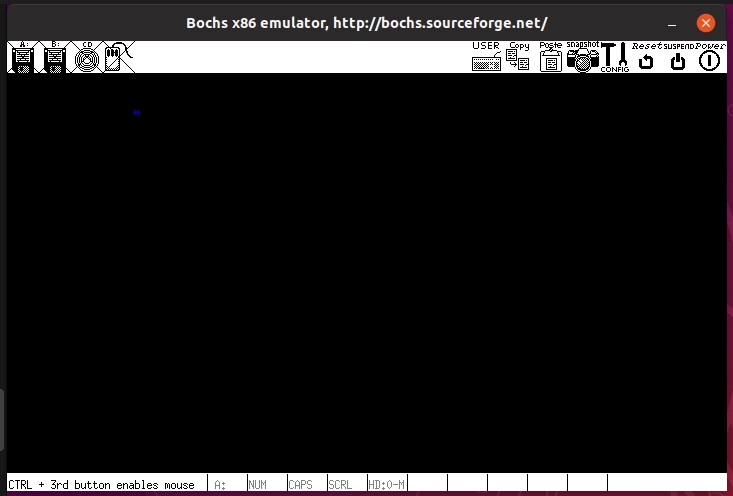
\includegraphics[width=15cm]{expr_image/1.png}
		\bottomcaption{软中断0x12}
	\end{figure}
	\begin{figure}[htbp]
		\centering
		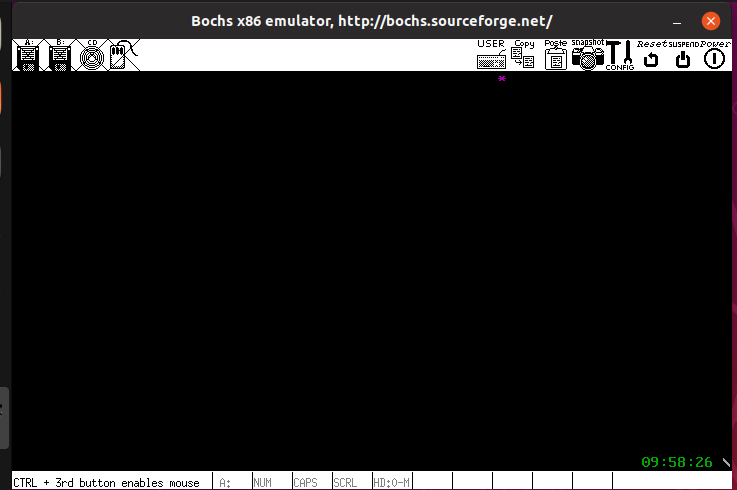
\includegraphics[width=15cm]{expr_image/2.png}
		\bottomcaption{}
	\end{figure}
	\begin{figure}[htbp]
		\centering
		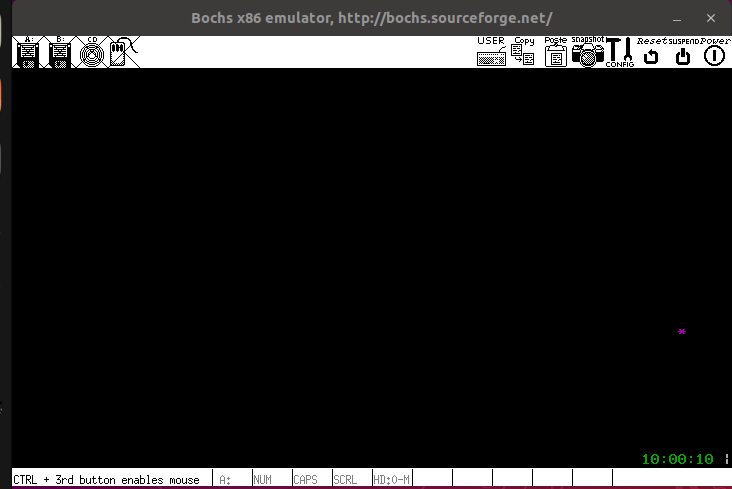
\includegraphics[width=15cm]{expr_image/3.png}
		\bottomcaption{}
	\end{figure}
	
	\begin{figure}[htbp]
		\centering
		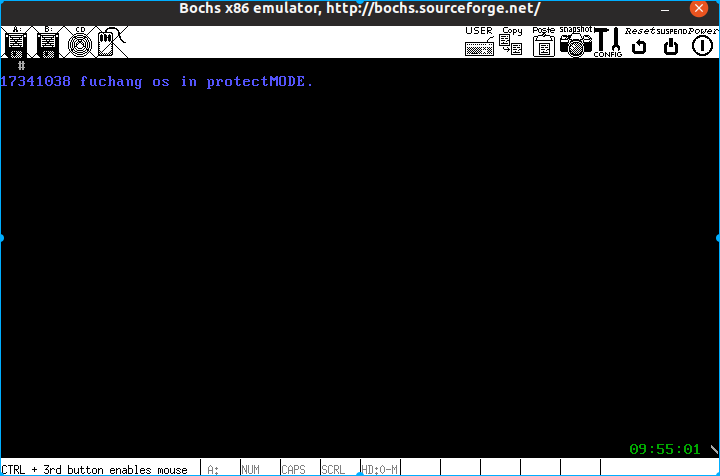
\includegraphics[width=15cm]{expr_image/DeepinScrot-5338.png}
		\bottomcaption{}
	\end{figure}
	
	\begin{figure}[htbp]
		\centering
		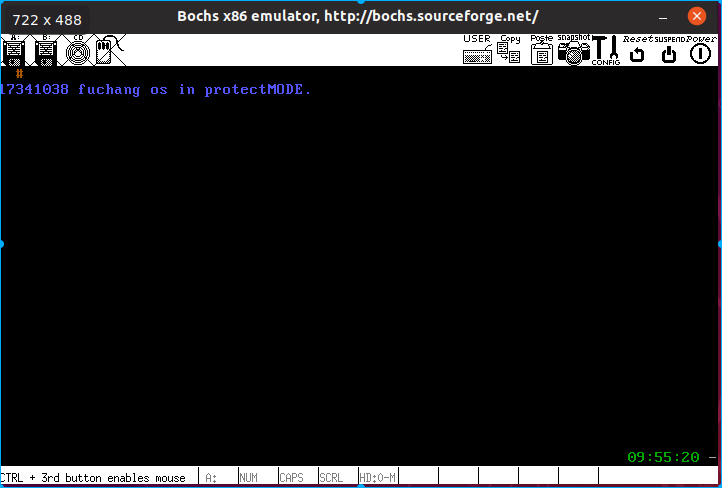
\includegraphics[width=15cm]{expr_image/DeepinScrot-5455.png}
		\bottomcaption{}
	\end{figure}

	\begin{figure}[htbp]
		\centering
		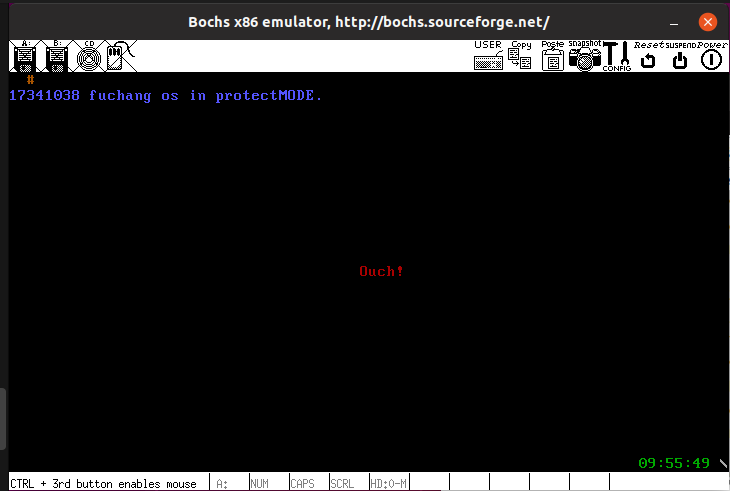
\includegraphics[width=15cm]{expr_image/4.png}
		\bottomcaption{}
	\end{figure}
	
	\begin{figure}[htbp]
		\centering
		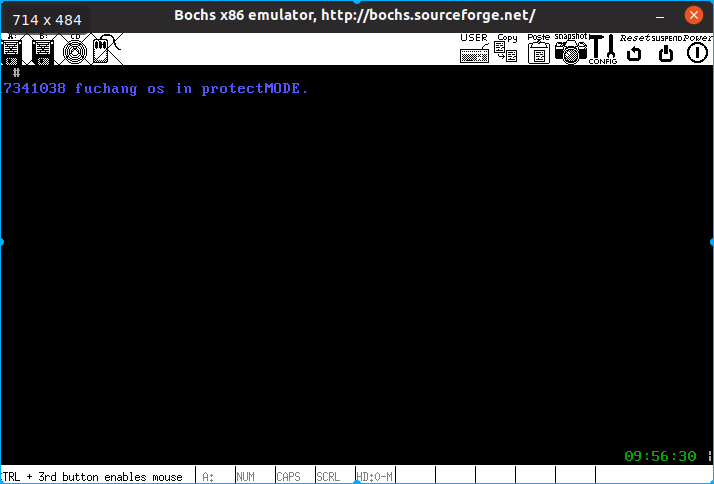
\includegraphics[width=15cm]{expr_image/DeepinScrot-5546.png}
		\bottomcaption{}
	\end{figure}
\section{实验总结}

\bibliographystyle{plain}
\bibliography{ref}

\clearpage



\end{document}
